\chapter{Blite-se}

Come già precedentemente detto il software realizzato può essere distinto
in due progetti a se stanti: \emph{Blite-se} e \emph{Blide}. In questo capitolo
si descrive il primo; sono presentati ad alto livello i diversi
moduli con le loro funzionalità e in particolare per l'Engine, il modulo predisposto all'esecuzione dei programmi
Blite, si descrive l'architettura in maniera dettagliata. Di questa si cerca di
mettere in luce il modello di esecuzione ideato, basato sul pattern
\emph{Composite} \cite{GANGo4}, secondo cui ogni attività è rappresentabile
come un componente che apporta il proprio contributo all'esecuzione dell'istanza di processo.

\section{Progetto di un motore per l'orchestrazione}

\label{sec:progmot}
\begin{figure}[t]
\begin{center}
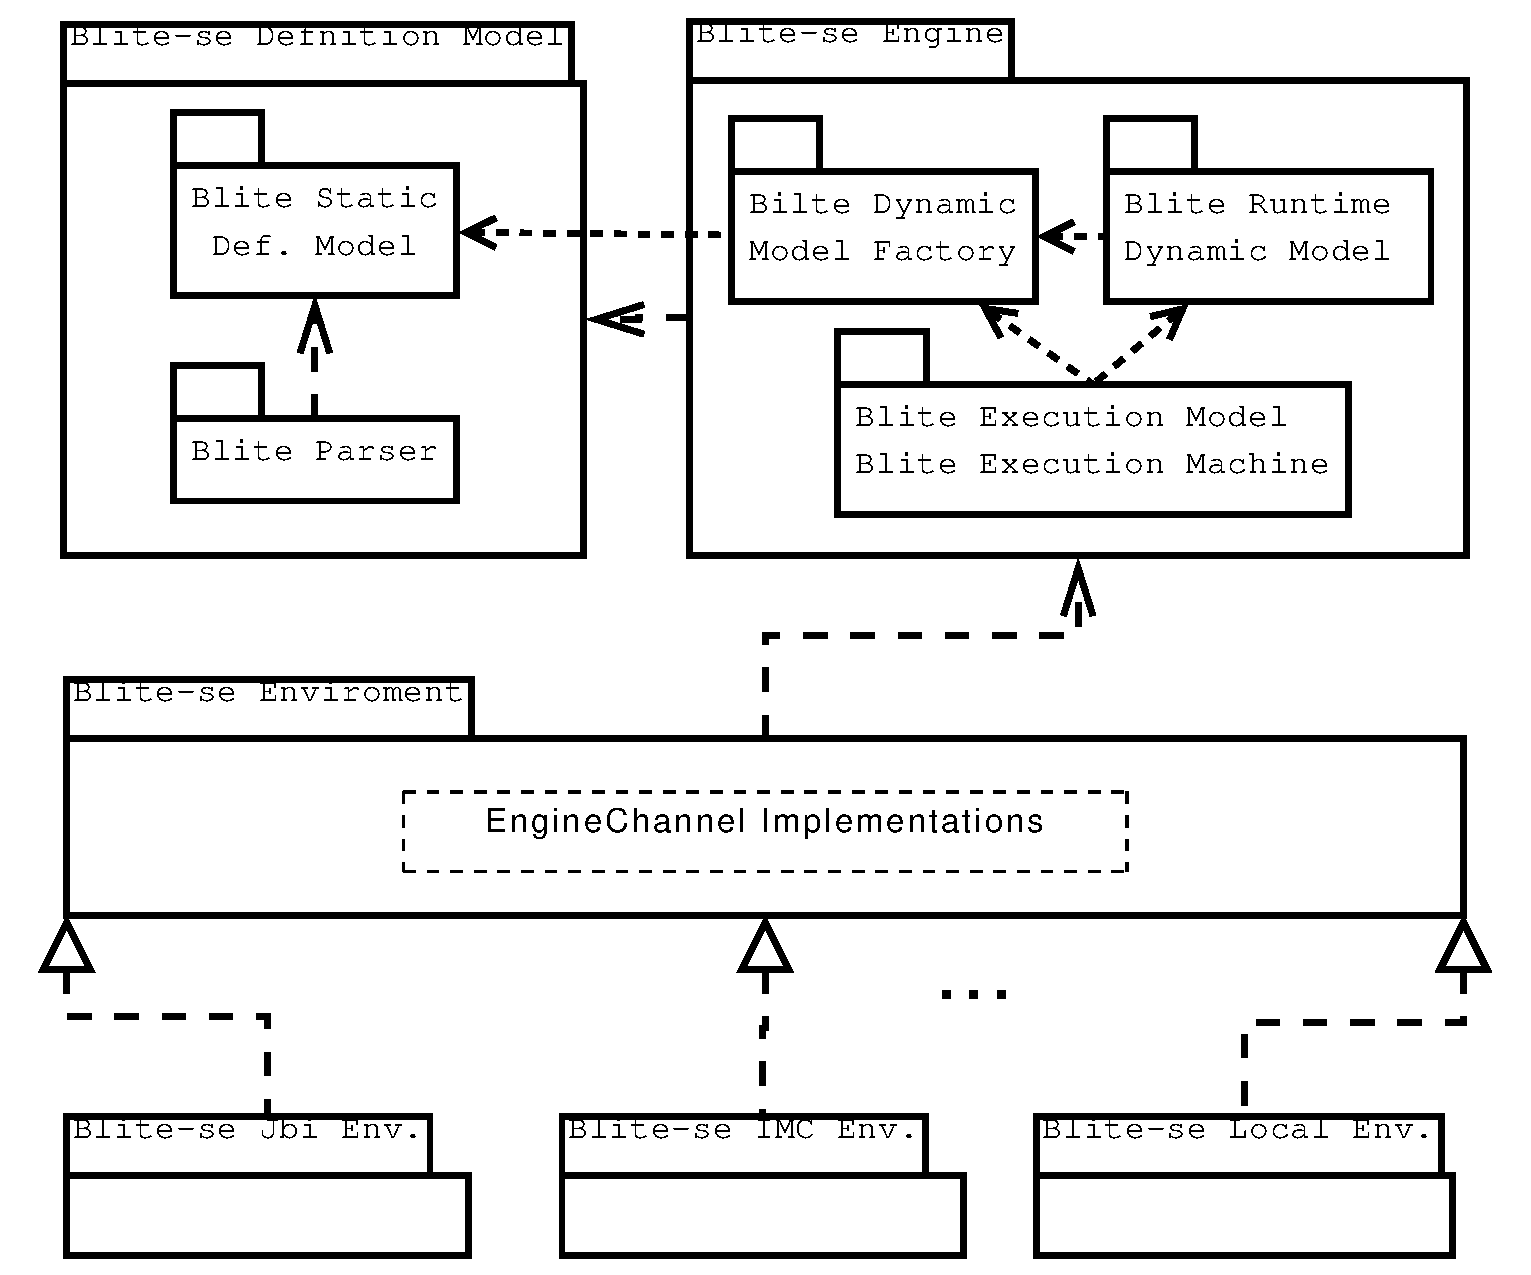
\includegraphics[scale=0.50]
{architettura_interna/dia/BliteModule}
\caption[I moduli di Blite-se] {I moduli software del progetto \emph{Blite-se}
e le loro dipendenze.}
\rule{7cm}{0.01cm}
  \label{fig:modules}
\end{center}
\end{figure}

Blite-se (Blite Service Engine) è il progetto principale e implementa il
linguaggio presentato nel capitolo precedente. Realizzare un linguaggio per
l'orchestrazione di servizi è un'attività complessa, che spazia in molteplici
aree dello sviluppo software. Per questo motivo è fondamentale organizzare il
progetto in moduli distinti che realizzino le diverse funzionalità in maniera
indipendente e che interagiscano fra loro con interfacce ben definite,
cercando di ridurre il più possibile le dipendenze dalle varie implementazioni.

Abbiamo individuato tre moduli principali con cui realizzare le funzionalità
necessarie:

\begin{enumerate}
  \item \emph{Blite-se Definition Model}: questo modulo realizza tutti quegli
  aspetti legati alla definizione statica dei programmi Blite. In pratica
  qui è definita la grammatica EBNF, secondo il formalismo di JJTree, da cui è 
  stato ricavato l'analizzatore sintattico. In questo modulo è realizzato anche
  il modello statico per i costrutti del linguaggio. Di fatto sono state
  implementate in maniera opportuna le classi i cui oggetti andranno a creare i
  nodi dell'albero sintattico. Tali classi sono tutte discendenti della classe
  \icode{BltDefBaseNode} che fornisce un'interfaccia comune per accedere ai
  rispettivi nodi padre e figli, inoltre fornisce il metodo:
	\begin{lstlisting}
		/** Accept the visitor. **/
		public Object jjtAccept(BliteParserVisitor visitor, Object data);
  	\end{lstlisting}  
  che permette la visita dell'albero secondo il pattern \emph{Visitor}
  \cite{GANGo4}. Oltre alle varie classi che implementano i nodi dell'albero sintattico  
  ovviamente è reso disponibile il parser tramite la classe \icode{BliteParser}.
  Questa dispone di due metodi statici\footnote{In JavaCC è stata usata
  l'opzione \textrm{STATIC = ``true''}, in questo modo il parser top-down a
  discesa ricorsiva è generato esclusivamente tramite metodi statici.
  L'efficienza risulta aumentata ma ovviamente, vi può essere un
  unico compilatore per virtual machine e successive compilazioni devono
  prevedere una di fase di reinizializzazione.}:
	\begin{lstlisting}	
		static public void init(java.io.InputStream stream)

		static public BltDefBaseNode parse() throws ParseException 
  	\end{lstlisting}
	che hanno le funzionalità rispettivamente di inizializzare il parser su una
	risorsa di input e di eseguire l'analisi sintattica su di questa. Il valore
	restituito dal metodo \icode{parse()} è ovviamente un oggetto conforme al
	tipo \icode{BltDefBaseNode} e nel caso specifico l'oggetto istanza della classe
	\icode{BLTDEFCompilationUnit} che costituisce la radice dell'albero
	rappresentante la struttura del programma Blite. Da osservare l'eccezione
	\icode{ParseException} eventualmente sollevata dal metodo \icode{parse()}; con
	essa è realizzata la gestione degli errori lessicali e sintattici incontrati
	durante una compilazione. Dai suoi metodi è possibile risalire a tutte le
	informazioni utili eventualmente per correggere l'errore, come: il token
	corrente, i token attesi, la riga e la colonna a cui si è arrestata la
	compilazione.
	
	Questo modulo non dipende dagli altri, ma da questi sarà utilizzato.
	
  \item \emph{Blite-se Environment}: questo modulo ha lo scopo di realizzare
  l'ambiente contenitore per l'Engine, facendo sì che nella realizzazione di
  quest'ultimo si possa astrarre dagli aspetti più tecnologici come le
  problematiche di comunicazione o di deployment. Di fatto si vuole
  che il motore di esecuzione possa essere utilizzato in scenari
  diversi e questo modulo realizza le astrazioni necessarie per rendere
  indipendente l'engine dalle diverse tecnologie di comunicazione. Per esempio
  una possibilità molto interessante potrebbe essere quella di integrare
  l'engine Blite con un ESB (Enterprise Service Bus) basato sul protocollo JBI,
  in questo caso basterebbe realizzare un sottomodulo con le funzionalità
  specifiche per dialogare con il bus. Un'altra ancora potrebbe essere
  quella di realizzare un environment capace di supportare direttamente gli
  standard tipici della tecnologia Web Services, come WSDL, SOAP e HTTP, e
  poter quindi far dialogare i nostri programmi Blite con ogni servizio di Internet. 
  Attualmente è stato implementato un environment (\emph{Local Environment})
  capace di eseguire localmente più Engine e simulare
  la rete e la comunicazione remota. Tale environment è stato creato per 
  realizzare i test di verifica dell'implementazione dell'Engine\footnote{Nel
  progetto Local Environment è stata realizzata una \emph{Test Suite} basata su \emph{JUnit}
  in cui vengono verificate le attività e i costrutti del linguaggio con
  test eseguiti nell'ambiente locale.}, e per allestire l'ambiente di esecuzione
  di \emph{Blide}, strumento nato per fare prototipi e simulazioni di processi.
  
  A livello di Engine è definita e utilizzata la seguente interfaccia
  \icode{EngineChannel}:
	\begin{lstlisting}
	/**
	 * This interface represents the communication channel between 
 	 * the Engine and the Environment.  
 	 * 
 	 * @author panks
 	 */
	public interface EngineChannel {
		
   		/**
      	 * This method initializes a communication exchange from 
     	 * the invoking process to the requested endpoint
     	 * 
         * @param serviceId
     	 * @param operation
     	 * @param messageContainer
     	 * @param instance the Process Instance initiating the exchange.
     	 * 
     	 * @return Object messageExchangeId 
     	 *         the identification key for communication protocol state .
     	 *         
     	*/
     	public Object createExchange(ServiceIdentifier serviceId, 
        	                         String operation,
            	                     ProcessInstance instance);
   
    	/**
     	 * Send a message container into the created exchange. 
     	 * This a creation post step in the communication.
     	 * 
     	 * @param messageContainer, the conteiner for application message e
         *        possible metadata.
         * @param messageExchangeId the identification key for communication 
	     *        protocol exchange.
     	 */
    	public  void sendIntoExchange(Object messageExchangeId,
                                      MessageContainer messageContainer);

    	/**
     	 * Closes the exchange.
     	 * 
     	 * @param messageExchangeId
     	 */
    	public void closeExchange(Object messageExchangeId);
	}

  	\end{lstlisting} 

	Tramite questa, la parti del motore di esecuzione interessate alla
	comunicazione, potranno inizializzare, sviluppare e concludere le comunicazioni
	con l'Environment; quest'ultimo invece utilizzerà l'interfaccia dell'Engine
	stesso per instradare le richieste, che dall'esterno, arriveranno verso
	le porte dei programmi Blite.
	
	Da osservare come tale interfaccia definisca un modello di comunicazione
	totalmente generico, che può essere utilizzato per realizzare molteplici
	protocolli per lo scambio di messaggi, dal più semplice \emph{``fire and
	forget''} ai più complessi, che necessitano un mantenimento dello stato.
	Alla base di questo ci sono l'astrazione \icode{MessageContainer}, che
	permette di raggruppare i messaggi applicativi con eventuali
	metainformazioni, e il \icode{messageExchangeId}, che costituisce un
	identificativo univoco per la sessione corrente di comunicazione.
	
	Le varie tipologie di Environment implementeranno in maniera opportuna tale
	interfaccia in modo da supportare la tecnologia di comunicazione desiderata.
	L'enviroment dopo aver creato le istanze della classe Engine imposterà in esse
	l'oggetto che realizza l'opportuna implementazione di
	\icode{EngineChannel}. Il modulo dipende da \emph{Blite-se Definition Model}
	per svolgere le funzionalità di compilazione e deploy, e ovviamente da
	\emph{Blite-se Engine} per la realizzazione delle esecuzioni.
	
  \item \emph{Blite-se Engine}: questo modulo contiene l'implementazione vera
  e propria del motore di esecuzione per i programmi Blite. Esso potrà essere
  eseguito all'interno di un opportuno Environment e, nel caso in cui
  quest'ultimo supporti la comunicazione remota, essere istallato su un nodo di
  rete per rendere disponibili i processi Blite ai client. Nei
  paragrafi successivi di questo capitolo verrà illustrata nel dettaglio
  l'architettura di questa parte di software. Questo modulo utilizza il
  \emph{Blite-se Definition Model} per accedere al modello statico
  rappresentante la definizione dei programmi Blite.
  
\end{enumerate}

In Figura \ref{fig:modules} è illustrato un diagramma (senza un
formalismo specifico) che rappresenta i vari moduli e le loro dipendenze.
\newpage

\section{Specifica dell'Engine}

In uno scenario reale, in cui i processi sono distribuiti, avremo un Engine per
locazione o, nodo di rete, e su ognuno di questi componenti sarà possibile
istallare o rimuovere definizioni di processi Blite. In pratica un engine
gestir\`a un insieme di definizioni, creando a partire da queste istanze di
processi e utilizzerà l'Environment per interagire con gli altri Engine. 
Dall'Environment stesso l'Engine riceverà notifiche riguardo l'accadere di
eventi, quali l'arrivo di messaggi indirizzati alle porte delle sue definizioni.

Dal punto di vista logico relazionale abbiamo già individuato le
macro entità e relazioni rappresentate in Figura \ref{fig:1}.

\begin{figure}[th]
\begin{center}
  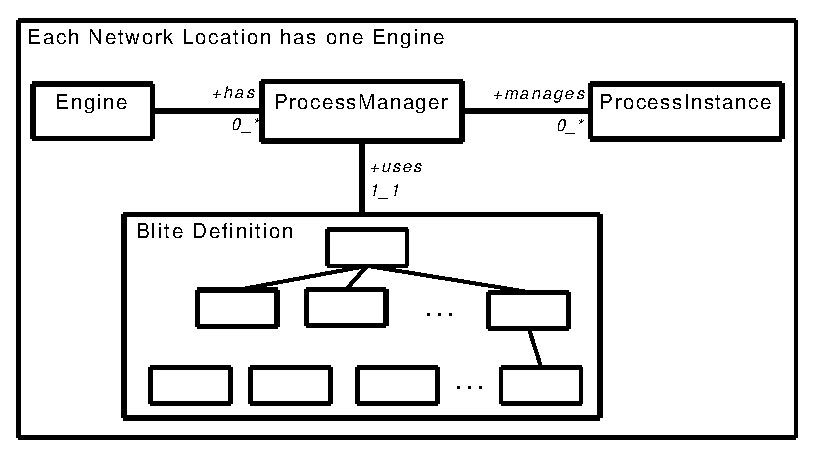
\includegraphics{architettura_interna/dia/engine}
  \caption[Blite-se: Engine, ProcessManager e ProcessInstace]{
  	Un Engine, ha $n$ definizioni di processo e per ognuna di esse un
  	\icode{ProcessManager}. Questo gestisce le \icode{ProcessInstace}
  	istanziandole dalla definizione.}
   \rule{7cm}{0.01cm}
  \label{fig:1}
\end{center}
\end{figure}

Per ogni definizione istallata sull'Engine sarà presente un oggetto 
della classe \icode{ProcessManager} che avrà il compito di gestire, nel loro
ciclo di vita, le istanze di processo derivate dalla definizione.

Prima di entrare nel dettaglio delle scelte architetturali ricapitoliamo quali
sono le caratteristiche peculiari di un sistema che deve gestire programmi per
l'orchestrazione di servizi, in modo che sia pi\`u facile da una parte
comprendere e dall'altra giustificare le scelte fatte.

A nostro vantaggio abbiamo che: \nopagebreak
\begin{itemize}
  \item Un Engine contiene in generale un numero contenuto di definizioni, per
  cui non ci interessa la scalabilità rispetto alla quantità di definizioni
  istallate su singolo engine. Tale scalabilità al contrario può essere
  ottenuta aggiungendo altri engine e installando definizioni su engine diversi.
  
  \item  Una definizione (o programma) Blite avendo principalmente funzionalità
  di integrazione avrà una lunghezza generalmente limitata. 
  
  \item Poiché le operazione fondamentali di un programma di questo genere
  sono invocazioni remote, le durate delle esecuzioni hanno ordini di grandezza
  minimi dettati dai tempi caratteristici della rete. Per questo motivo non
  risulta determinante l'efficienza di esecuzione delle operazioni interne di un
  processo. Il nostro engine non necessiterà di una particolare ottimizzazione 
  rispetto all'efficienza di esecuzione interna.
\end{itemize}

Al contrario, risultano particolarmente critici i seguenti aspetti:
\begin{itemize}
  \item Per ciascuna definizione potrà essere richiesta la creazione di
  numerose istanze. La scalabilità rispetto al numero delle
  richieste remote e quindi di istanze di processo risulta essere un
  prerequisito fondamentale.
  
  \item Se da un lato abbiamo detto che l'efficienza di esecuzione non \`e 
  un aspetto particolarmente critico, dall'altro per\`o ogni attività interna
  necessita di un elevato grado di controllo e tracciabilità. Ogni attività deve
  potere essere eventualmente terminata o abortita. Poiché in generale
  ogni istanza potrebbe avere un'immagine persistente o
  perlomeno essere soggetta ad una attività di monitoring, l'Engine necessiterà
  di un grado di controllo a livello di singola attività Blite.
\end{itemize}

Tenendo conto di queste iniziali considerazioni sono state fatte alcune scelte
basilari di organizzazione del progetto e l'architettura software \`e stata
basata sulle seguenti specifiche fondamentali:

\begin{enumerate}
  \item La compilazione di una definizione Blite (che eventualmente in un
  ambiente distribuito può essere fatta in fase di deploy) produce un modello
  statico della definizione stessa, che può essere implementato con
  una struttura ad oggetti. Tale struttura può essere mantenuta in memoria
  presso l'Engine e esplorata a runtime per ricavare il
  flusso e la logica di esecuzione. Sempre in fase di deploy l'Engine può
  ricavare tutte le informazioni per popolare le strutture dati in cui sono 
  memorizzati i binding fra i nomi delle porte e le definizioni; anche tali
  strutture dati possono essere mantenute in memoria.
  
  \item Le richieste che giungono all'Engine non devono produrre un aumento
  delle risorse complessive mantenute dall'Engine. Ogni istanza di processo nel
  suo svolgersi deve, man mano che procede, rilasciare le risorse di memoria
  acquisite. Anche il numero complessivo dei thread deve essere limitato
  superiormente (generalmente dell'ordine dell'unità). La realizzazione del
  parallelismo di attività deve essere attuata tramite il pattern ``Resources
  Pool'': ogni Engine deve disporre di un pool di thread con cui eseguire in
  parallelo le attività secondo le definizioni Blite.
  
  \item Il modello di esecuzione deve essere Activity Centric. L'engine deve
  trattare ogni attività secondo un'astrazione generica che possa permettere di
  fattorizzare i comportamenti comuni e mantenere semplice e pulita
  l'implementazione della semantica di esecuzione del linguaggio.
\end{enumerate}

%%%%%%%%%%%%%%%%%%%%%%%%%%%%%%%%%%%%%%%%%%%%%%%%%%%%%%%%%%%%%%%%%%%%%%%%%%%%%%%%
%						Modello per l'Attività
%%%%%%%%%%%%%%%%%%%%%%%%%%%%%%%%%%%%%%%%%%%%%%%%%%%%%%%%%%%%%%%%%%%%%%%%%%%%%%%%
\section{Un modello per le attività}
A questo punto, dopo aver esposto a grandi linee quelle che devono essere le
caratteristiche fondamentali di un Engine, entriamo nel dettaglio del progetto
dell'architettura. Nella realizzazione di questa abbiamo scelto di utilizzare
il formalismo degli oggetti e delle classi secondo il consueto paradigma
``Object Oriented''. Inoltre abbiamo preso come fonte di
ispirazione il pattern \emph{Composite} \cite{GANGo4} cercandone una
trasposizione nella problematica dell'esecuzione di un programma Blite. In particolare
l'astrazione di componente \`e stata applicata all'entità ``attività''. Come i
componenti contribuiscono alla realizzazione di un documento o di una
interfaccia utente, le singole attività contribuiscono allo svolgersi
dell'esecuzione di un processo Blite.
 
Inoltre la tipica struttura gerarchica presente staticamente negli elementi
sintattici di una definizione può essere naturalmente riprodotta a runtime tra
i singoli passi di esecuzione, andato a completare l'analogia con le strutture
gerarchiche ad albero tipiche dei tradizionali domini di applicazione del
Composite Pattern. 

L'entità fondamentale del nostro dominio applicativo \`e stata quindi
individuata nella \icode{ActivityComponent}, trasposizione a runtime
dell'elemento sintattico Activity definito dalla grammatica di Blite.
Ogni \icode{ActivityComponent} \`e rappresentabile tramite 
interfaccia del Listato \ref{lst:ActivityComponent} e descritta in Tabella \ref{it:actcomp}.

\lstinputlisting
[caption={Interfaccia base del modello di escuzione dell'Engine Blite},
label=lst:ActivityComponent]
{architettura_interna/java/ActivityComponent.java}

\begin{table}[t]
\begin{center}

\begin{tabular}{| p{0.3\textwidth } | p{0.6\textwidth}|}
\hline
\icode{ActivityComponent} &  \\
\hline
\small{\icode{boolean doActivity()}} & \small{Costituisce il metodo
centrale per lo svolgersi dell'esecuzione del programma. L'invocazione di tale 
metodo su un oggetto attività fa si che essa possa essere eseguita. Il valore
booleano restituito sarà il discriminante del fatto che il flusso di esecuzione
corrente dovrà o meno interrompersi. Ogni attività oltre che eseguire se
stesa sarà quindi anche responsabile nel guidare il flusso nel passo
successivo. Utilizzando la gerarchia ad essa nota imposterà la nuova attività
corrente da eseguire (l'attività padre o figlio) e restituirà il valore
true. Al contrario, potrà interrompere il flusso corrente restituendo false.
}\\
 
& \\
\small{\icode{ActivityComponent \linebreak 
\hspace*{\stretch{3}} getParentComponent()}} & \small{Tale metodo restituisce
 l'elemento padre dell'attività corrente. In questo modo si realizza la struttura gerarchica fra
i vari componenti dell'esecuzione.}\\
& \\
\small{\icode{BltDefBaseNode \linebreak  \hspace*{\stretch{3}} getBltDefNode()}}
& \small{Ogni attività componente dell'esecuzione \`e strettamente 
associata ad un elemento sintattico del programma. Con questo metodo ogni 
oggetto attività restituisce il nodo che la definisce nell'albero sintattico
ricavato dal parsing del codice Blite.}\\

\hline
\end{tabular}
\caption{Metodi principali dell'interfaccia \icode{ActivityComponent}}
\label{it:actcomp}
\end{center}
\end{table}

\begin{figure}[t]
\begin{center}
  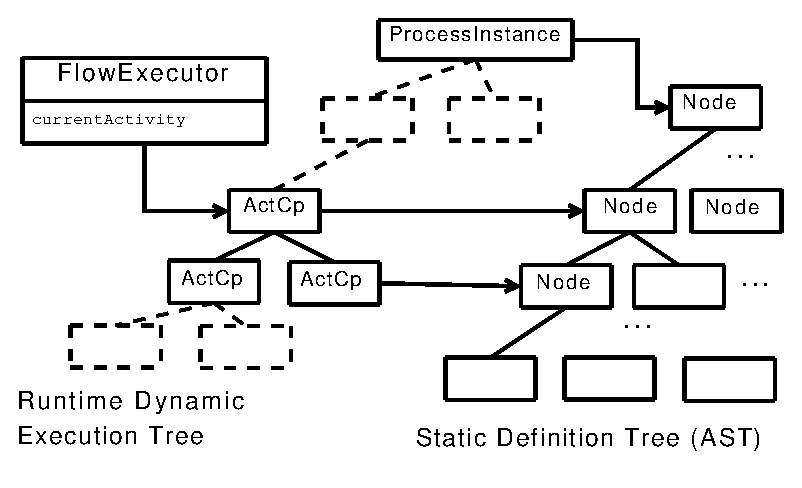
\includegraphics{architettura_interna/dia/tries}
  \caption[Blite-se: modello statico e modello dinamico]{Il modello statico è
  utilizzato a runtime per costruire il modello dinamico delle
  \icode{ActivityComponent}.}
   \rule{7cm}{0.01cm}
  \label{fig:2}
\end{center}
\end{figure}

Lo scenario che si va a delineare \`e quindi quello di due strutture gerarchiche
associate: una costituita dall'AST (Abstract Syntax Tree) ricavato dal parsing
del codice Blite, e che come si detto \`e mantenuta nella sua interezza, l'altra
costituita dall'albero dinamico delle ActivityComponent che realizzano
l'esecuzione a runtime (Figura \ref{fig:2}). Quest'ultima struttura, una per ogni
istanza, non \`e però costruita in un unico momento in fase di inizializzazione
del  processo, ma al contrario \`e istanziata man mano che l'esecuzione procede. 
Come già accennato le attività stesse avranno il compito di creare i loro
successori e di metterli in esecuzione. Inoltre gli oggetti attività già eseguiti
dovranno essere rilasciati il prima possibile in modo da poter essere
collezionati dal Garbage Collector e rilasciare le risorse di memoria.



Per ogni tipologia di attività prevista dalla grammatica di Blite esiste
una sottoclasse specifica che implementa l'interfaccia
\icode{ActivityComponent} e che realizza in maniera opportuna, in rispetto
della semantica, il metodo \icode{boolean doActivity()}. 
Per ottimizzare il disegno e fattorizzare
il codice comune \`e stata ovviamente introdotta una classe astratta
\icode{ActivityComponentBase} da cui ogni altra implementazione di
\icode{ActivityComponent} eredita le funzionalità comuni di base.

Anche la classe \icode{ProcessInstance}, che modella con i suoi oggetti le
varie istanze di processo nell'engine, implementa l'interfaccia
\icode{ActivityComponent} uniformando la struttura gerarchica di esecuzione
(anche le attività che avranno come padre oggetti
\icode{ProcessInstance} potranno interagire con questi tramite l'interfaccia
\icode{ActivityComponent}).

Le varie istanze di \icode{ActivityComponent} del tipo specializzato verranno
create tramite una classe Factory \icode{ActivityComponentFactory}, Listato
\ref{lst:ActivityComponentFactory}, che espone il metodo
\icode{ActivityComponent makeRuntimeActivity($\cdot$)}. In Tabella
\ref{it:fact} è descritta la segnatura di tale metodo.
 
\lstinputlisting
[caption={ActivityComponentFactory, permette di creare oggetti
ActivityComponent}, label=lst:ActivityComponentFactory]
{architettura_interna/java/ActivityComponentFactory.java}

In Figura \ref{fig:actclass} viene riportato un diagramma di classe
abbastanza dettagliato per le entità \icode{ActivityComponent}.

\begin{table}
\begin{center}
\begin{tabular}{| p{0.5\textwidth } | p{0.4\textwidth}|}
\hline
\icode{ActivityComponentFactory} & \\
\hline

\small{
\icode{ActivityComponent \linebreak makeRuntimeActivity( 
\linebreak \hspace*{\stretch{3}} BltDefBaseNode bltDefNode, 
\linebreak \hspace*{\stretch{3}} ExecutionContext context, 
\linebreak \hspace*{\stretch{3}} ActivityComponent parentComponent, 
\linebreak \hspace*{\stretch{3}} FlowExecutor executor)}} 
& \small{Permette di ottenere istanze opportune di oggetti
\icode{ActivityComponent}. Il parametro bltDefNode individua l'elemento
sintattico che definisce l'attività specifica, in pratica il nodo nell'AST.
Il parametro parentComponent l'attività padre nella gerarchia di esecuzione,
mentre gli altri due parametri individuano rispettivamente il contesto di
esecuzione e l'esecutore del flusso in cui l'attività verrà creata. Tali
entità verranno descritte nelle sezioni successive}\\
\hline
\end{tabular}
\end{center}
\caption{Factory per creare le opportune sottoclassi che implementano le
attività}
\label{it:fact}
\end{table}

\begin{figure}[p]
\begin{center}
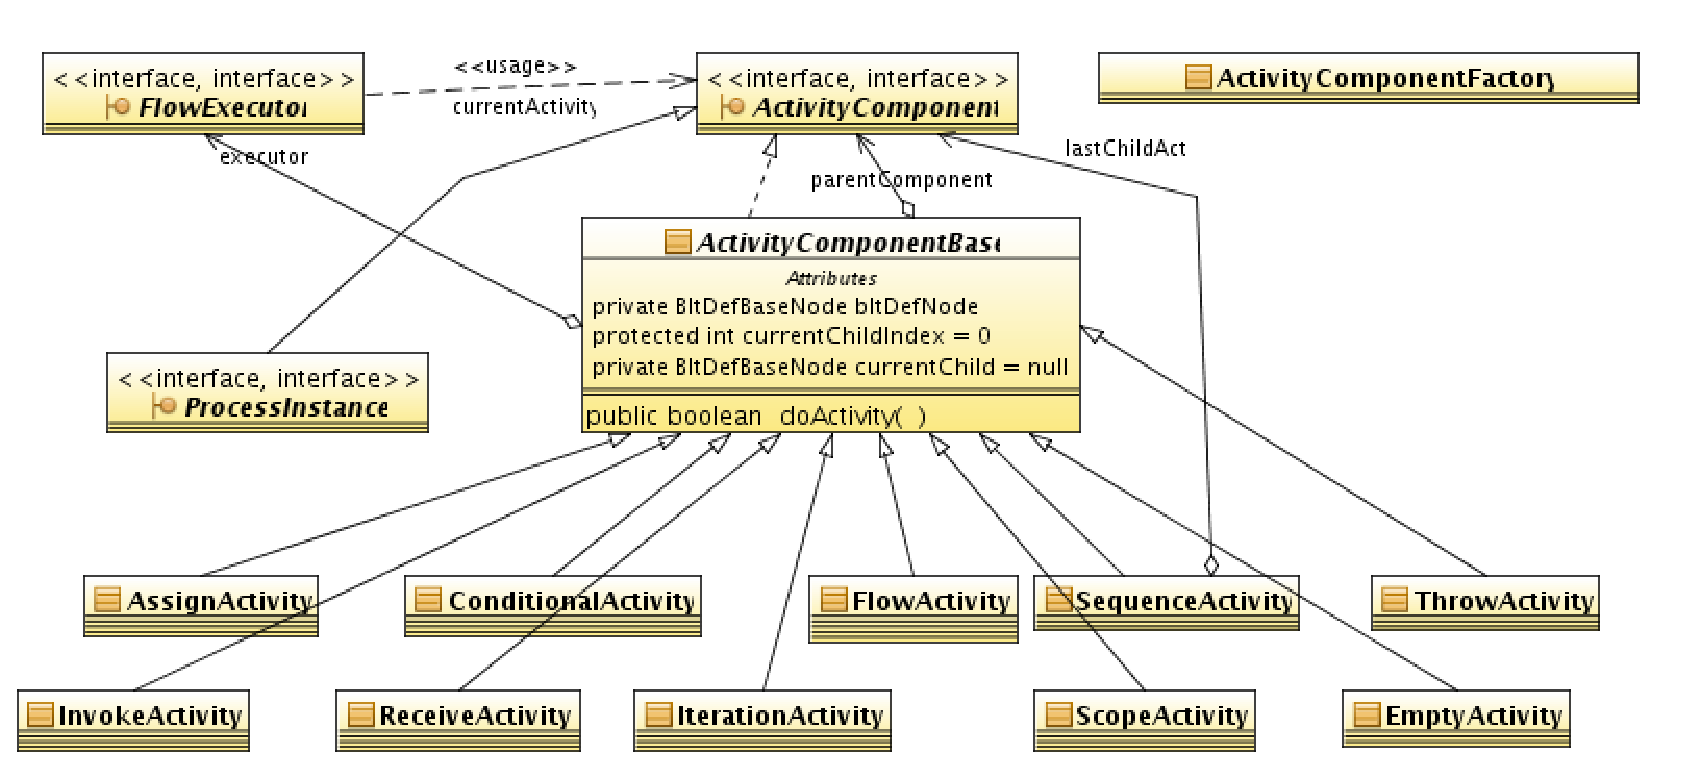
\includegraphics[angle=90,scale=0.75]
{architettura_interna/dia/actclass}
\caption[Blite-se: Gerarchia delle ActivityComponent]{
   	Diagramma di classe per la gerarchia delle
   	\icode{ActivityComponent}}
  \label{fig:actclass}
\end{center}
\end{figure}

\newpage
% %%%%%%%%%%%%%%%%%%%%%%%%%%%%%%%%%%%%%%%%%%%%%%%%%%%%%%%%%%%%%%%%%%%%%%%%%%%%%%%
% Esecuzione e parallelismo
% %%%%%%%%%%%%%%%%%%%%%%%%%%%%%%%%%%%%%%%%%%%%%%%%%%%%%%%%%%%%%%%%%%%%%%%%%%%%%%%
\section{Esecuzione e parallelismo}
Abbiamo visto che i componenti base per l'esecuzione sono oggetti delle varie
sottoclassi che implementano l'interfaccia \icode{ActivityComponent} e che
l'esecuzione ha atto tramite l'invocazione del metodo
\icode{doActivity()} su tali oggetti. A questo punto però dobbiamo
domandarci da chi e in che modo tale metodo è invocato. Nel rispondere a questa
domanda dobbiamo tenere conto che in un Engine verranno eseguite
contemporaneamente molteplici istanze di processo e che inoltre il formalismo
stesso del linguaggio dà la possibilità di richiedere l'esecuzione concorrente
di diverse attività (costrutto flow). Quindi su ciascun Engine dovranno essere
disponibili più thread per poter realizzare un livello di
parallelismo sufficiente.

Si capisce bene che istanziare un nuovo oggetto Thread per ogni nuovo flusso
logico presente sull'engine non sia un approccio assolutamente vantaggioso. Come
già accennato infatti tale politica non sarebbe per nulla scalabile rispetto al
numero delle richieste remote gestite dell'engine; inoltre, poiché ogni istanza
di processo tendenzialmente trascorrerà la gran parte del suo tempo in attesa di
comunicazioni remote\footnote{Come già osservato i tempi di comunicazione remota
sono di vari ordini di grandezza maggiori rispetto a quelli delle operazioni
interne per cui ogni istanza nel suo ciclo di vita si troverà ad occupare
realmente la CPU per tempi quasi trascurabili rispetto ai tempi di attesa di
eventi remoti.}, ci troveremmo con un gran numero di thread in stato di attesa,
con uno spreco di risorse del tutto ingiustificabile. Più banalmente gestire
direttamente oggetti Thread \`e una pratica alquanto sconsigliabile
\footnote{Questo \`e ancor pi\`u vero dalla versione 5 in poi di Java, in cui
sono stati introdotti i pacchetti \icode{java.util.concurrent.*} che mettono a
disposizione un framework ad alto per la concorrenza livello che ottimizza e
astrae l'uso delle API a più basso livello.}, in quanto può portare ad errori di
programmazione o a Memory Leaks nel caso in cui il ciclo di vita di tali oggetti
non sia sempre ben gestito dal programmatore. Per questi motivi si \`e scelto di
utilizzare la tecnica del Pooling per gestire un insieme di Thread a livello di
Engine. Con tale tecnica si isola la gestione della tecnologia di multitasking e
si possono applicare politiche anche molto raffinate capaci di adattare la
quantità di risorse utilizzate al carico di lavoro da svolgere. Nella
implementazione attuale dell'Engine si \`e fatto uso dei thread pool forniti
dalla classe \icode{java.util.concurrent.Executors} presente nella piattaforma
standard Java 5.
 
La scelta che quindi \`e stata fatta per realizzare il parallelismo \`e la
seguente: ogni flusso logico attivo presente nelle varie istanze di processo sarà
associato all'entità \icode{FlowExecutor} (tale entità \`e già comparsa in alcuni
diagrammi precedentemente illustrati in questo capitolo, per cui il lettore avrà
già intuito la sua funzionalità). Tali oggetti presentano l'interfaccia
descritta dal Listato \ref{lst:FlowExecutor}, essa permette da un lato di
impostare l'attività corrente che dovrà essere eseguita da uno dei thread del pool, 
dall'altro di eseguire effettivamente tale attività.

\lstinputlisting
[caption={I FlowExecutors saranno gli oggetti che realizzeranno i flussi di
esecuzione parallela all'interno dell'Engine }, label=lst:FlowExecutor]
{architettura_interna/java/FlowExecutor.java}

A questo punto, quando ci sarà bisogno di creare un nuovo flusso di esecuzione
per l'ActivityComponent \texttt{act} si dovrà creare un nuovo FlowExecutor
impostarvi \texttt{act} come attività corrente e renderlo disponibile ad un thread per
l'esecuzione. Quest'ultimo passaggio verrà realizzato tramite l'interfaccia
dell'Engine che dispone del seguente metodo per notificare gli executor pronti
per essere eseguiti e metterli a disposizione del pool di thread:

\lstinputlisting {architettura_interna/java/queueFlowExecutor.java}

Inoltre quando un flusso giungerà a conclusione (l'istanza di processo termina o
una esecuzione parallela definita in una flow Activity si conclude) si dovrà
registrare tale evento e produrre eventualmente altri effetti. Per far si che si
realizzi questa necessità si \`e introdotto il concetto di \icode{FlowOwner},
Listato \ref{lst:FlowOwner}. Ogni attività che nel suo eseguirsi si
troverà a creare nuovi flussi di esecuzione, e quindi oggetti \icode{FlowExecutor},  dovrà implementare
l'interfaccia \icode{FlowOwner} e impostare se stessa nel \icode{FlowExecutor}
da essa creato. In questo modo quando il flusso logico terminerà, il FlowOwner potrà
ricevere notifica di tale accadimento tramite l'invocazione del metodo
\icode{flowCompleted()}.

\lstinputlisting
[caption={Interfaccia \icode{FlowOwner}, gli oggetti che creeranno i flussi di
dovranno implementare tale interfaccia.}, label=lst:FlowOwner]
{architettura_interna/java/FlowOwner.java}

A questo punto \`e lecito domandarsi quando si dovrà considerare terminato un
flusso di esecuzione. In generale si applica il seguente ragionamento. Le varie
\icode{ActivityComponent}, che sono legate in una struttura gerarchica che
riflette la definizione statica del programma, termineranno la loro esecuzione
mettendo come attività corrente nel loro \icode{FlowExecutor} la propria attività
padre (\icode{parentComponent}). In accordo con questa osservazione risulta
quindi corretto affermare che un flusso di esecuzione può essere considerato
terminato dal \icode{FlowExecutor} quando questo si troverà ad eseguire come
attività corrente proprio il suo \icode{FlowOwner}. In questo caso su di esso il
FlowExecutor non dovrà invocare il metodo \icode{doActivity()} ma il metodo
\icode{flowCompleted()} e fatto questo, dovrà terminare di eseguire il flusso. Il
codice del Listato \ref{lst:FlowExecutorImp} spiega meglio di mille parole la
logica alla base di tutto il modello di esecuzione dell'Engine; in poche righe \`e sintetizzato il cuore
dell'architettura.

\lstinputlisting[caption={Classe che implementa il \icode{FlowExecutor}. Il
metodo \icode{executeCurrentActivity()} è il cuore del modello d'esecuzione
realizzato dall'Engine. Esso esegue l'attività corrente fintanto che essa non
sia uguale al \icode{FlowOwner}.},
label=lst:FlowExecutorImp]{architettura_interna/java/FlowExecutorImp.java}

In generale possiamo quindi dedurre le seguenti affermazioni che ci possono
aiutare a definire alcune proprietà invarianti.

\begin{itemize}
  \item Un FlowExecutor non invocherà mai il metodo \icode{doActivity} del suo
  FlowOwner. Viceversa, di questo potrà invocare il metodo
  \icode{flowCompleted()}.
  
  \item Su un oggetto ActivityComponent che implementa anche l'interfaccia
  FlowOwner, il metodo \icode{doActivity()} verrà invocato dal FlowExecutor
  dell'attività padre.
  
  \item Su di un oggetto ProcessInstance, che \`e il FlowOwner del flusso
  principale dell'istanza e che \`e l'unica attività senza padre, 
  il metodo \icode{doActivity()} non verrà mai invocato da nessun FlowExecutor.
  
  \item Il metodo \icode{doActivity()} di una ProcessInstance verrà invocato
  dall'Engine stesso in fase di creazione dell'istanza.
  
\end{itemize}

Oltre a creare, eseguire e terminare flussi sarà anche necessario sospenderne
alcuni già in esecuzione, si veda per esempio il caso dell'attività di ricezione
che deve arrestare il flusso corrente in attesa di un evento remoto. In questo
caso, l'attività utilizzando l'interfaccia dell'Engine e in particolare il
seguente metodo:

\lstinputlisting{architettura_interna/java/addFlowWaitingEvent.java}
potrà mettere in attesa il suo FlowExecutor su di un evento identificato dalla
chiave \texttt{eventKey} e che essa stessa aveva provveduto precedentemente a
ricavare\footnote{Si usa qui il termine ricavare, e non generare, in maniera
voluta. Le chiavi di evento non sono identificate da oggetti in memoria ma hanno
una loro entità indipendente
  dagli oggetti che posso essere creati per rappresentarle. Per un esempio le
  chiavi utilizzate per la ricezione saranno costituite dalla coppia
  $\langle \texttt{service-name}, \texttt{operation-name} \rangle$, tale coppia
  verrà indicata come \texttt{portId}.}. Fatto questo, l'attività ritornerà dal proprio
metodo doActivity con il valore false, in questo modo il FlowExecutor terminerà
l'esecuzione del Flow corrente. Nel momento in cui il messaggio sarà recapitato,
l'Engine potrà individuare il FlowExecutor tramite la chiave \texttt{eventKey} e
rimetterlo in esecuzione. Poiché l'attività corrente di quest'ultimo sarà rimasta
l'attività di ricezione, essa potrà riprendere la sue esecuzione, consumando il
messaggio e permettendo al suo flusso di esecuzione di procedere. Nella sezione
successiva verrà illustrato nel dettaglio come si realizza la comunicazione e la
notifica degli eventi.

\begin{figure}[!t]
\begin{center}
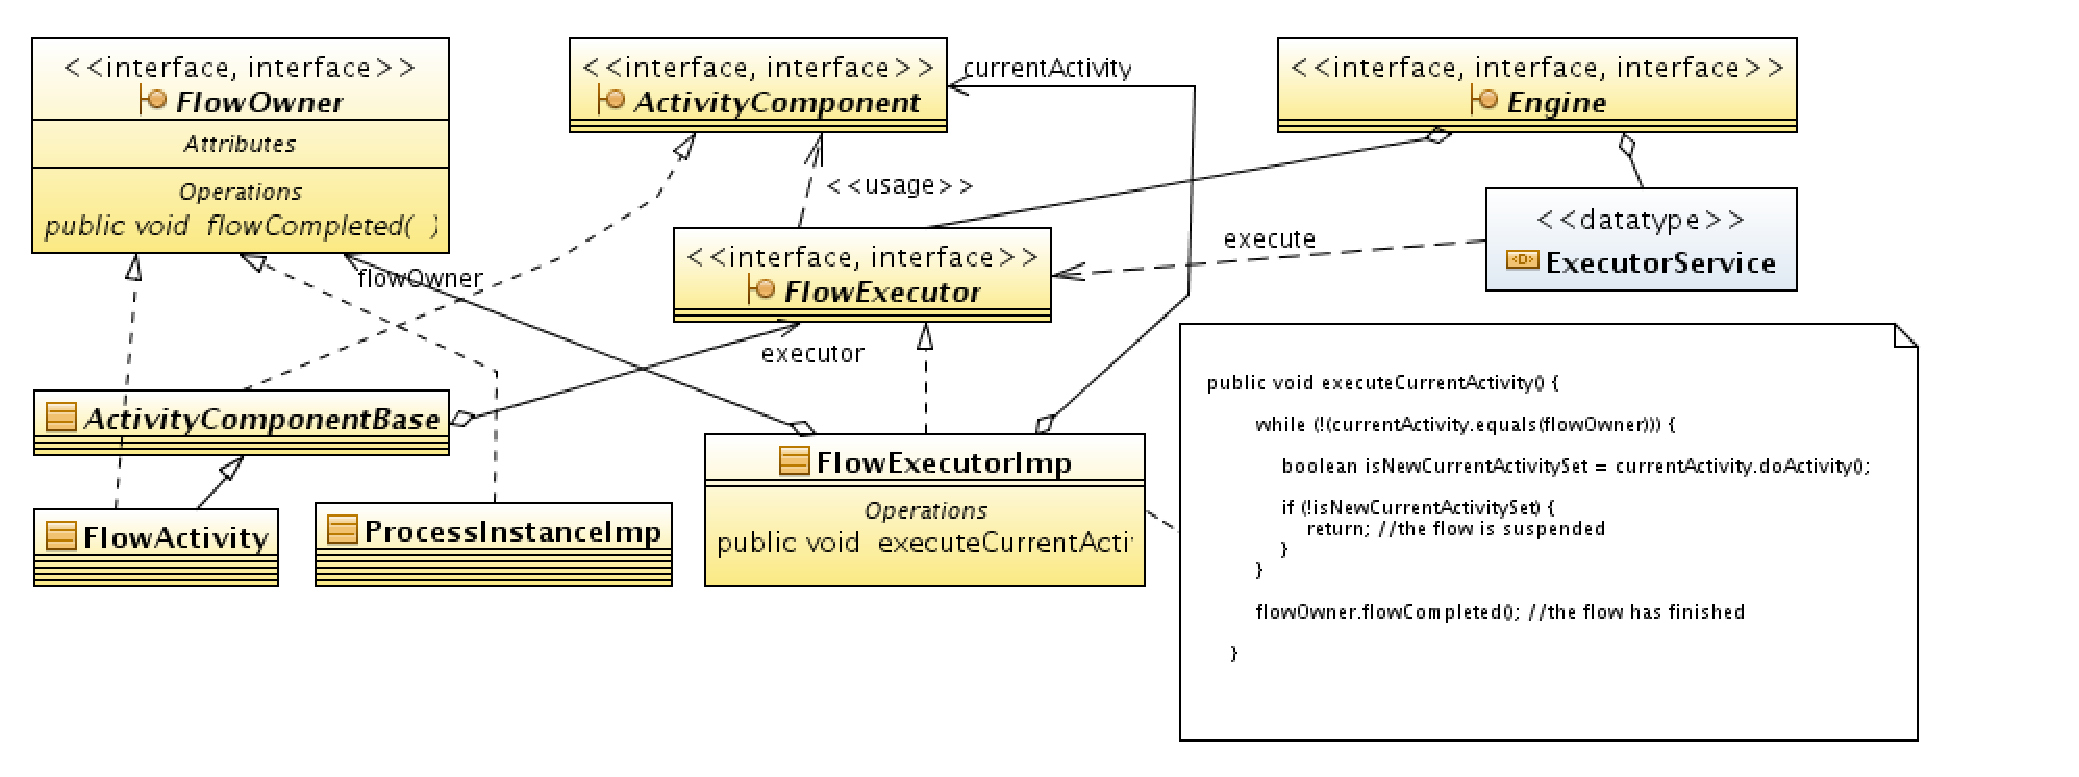
\includegraphics[angle=90,scale=0.626,clip]
{architettura_interna/dia/flowClassDiagram}
\caption[Diagramma di classe FlowExecutor \ldots] {
   	Diagramma di classe FlowExecutor, FlowOwner e ThreadPool}
  \label{fig:flowclass}
\end{center}
\end{figure}

In Figura \ref{fig:flowclass} \`e rappresentato un diagramma di classe che
raffigura, fra le altre entità, il FlowExecutor e FlowOwner e le principali
relazioni che le coinvolgono.

% %%%%%%%%%%%%%%%%%%%%%%%%%%%%%%%%%%%%%%%%%%%%%%%%%%%%%%%%%%%%%%%%%%%%%%%%%%%%%%%
% EVENTI E COMUNICAZIONE
% %%%%%%%%%%%%%%%%%%%%%%%%%%%%%%%%%%%%%%%%%%%%%%%%%%%%%%%%%%%%%%%%%%%%%%%%%%%%%%%
\section{Comunicazione ed eventi}
\label{sec:comevent}
Da quanto abbiamo già esposto risulta chiaro che l'esecuzione di un processo \`e
caratterizzata dallo svolgersi di attività interne e l'accadere di eventi
esterni di cui le attività possono essere in attesa. In generale si può
considerare che gli eventi sono generati a livello di Enviroment, e che possono
essere prodotti dall'arrivo di nuovi messaggi verso le porte locali o
dalla notifica degli ack/nok delle invocazioni locali
verso porte remote. Attualmente le funzionalità espresse da Blite non
individuano eventi diversi da queste due tipologie. Nell'Engine però si \`e
preferito realizzare un meccanismo generico di notifica di eventi che
soddisfacesse i requisiti attuali del linguaggio ma che non escludesse eventuali
possibilità di estensione verso altre caratteristiche tipiche di BPEL
(comunicazione Request-Response, EventActivity, ecc).

Per l'implementazione dello schema di comunicazione prescelto sono richieste
le seguenti funzionalità:

\begin{enumerate}
  \item A livello di attività o di ProcessManager stesso,
  sarà necessario ricavare una chiave univoca per uno specifico 
  evento. I tipi di evento e le regole per generare di volta in
  volta le chiavi verranno esposti di seguito. Per il momento può bastare aver
  chiaro che una chiave individua in maniera univoca una particolare tipologia di evento e all'interno di questa un evento specifico o un insieme
  di eventi gemelli.
  
  \item In un qualsiasi momento al ProcessManager potranno essere notificati
  eventi. In tal caso esso dovrà provvedere a ricavarsi la chiave e a
  memorizzare in una mappa associativa l'evento con la chiave per poterlo poi
  rendere disponibile alle attività interessate. Il ProcessManager dovrà anche
  provvedere a ``risvegliare'' tutti i flussi di esecuzione che
  eventualmente si sono messi in attesa di quell'evento specifico.
   
  \item In un qualsiasi momento, e anche più volte nel suo ciclo di vita, una
  attività potrà interrogare l'Engine (o meglio il ProcessManager responsabile
  della sua istanza) chiedendogli se un evento associato ad una particolare
  chiave sia avvenuto. In caso affermativo l'attività potrà consumare l'evento.

  \item Una attività potrà avere la necessità di mettersi in attesa di un
  particolare evento non ancora avvenuto, il tal caso dovrà sospendere il
  suo flusso di esecuzione e notificare questo al ProcessManager
  con il riferimento alla chiave dell'evento d'interesse. 
\end{enumerate}

% Tali funzionalità serrano rese disponibili nelle diverse interfacce 
% \ldots

In particolare si può vedere come queste funzionalità di base possono essere
utilizzate nel caso dell'attività \icode{ReceiveActivity}, e come
l'attività stessa collabora con il ProcessManager affinché si realizzi la
ricezione di messaggi. La \icode{ReceiveActivity} nel suo metodo
\icode{doActivity()} compierà i seguenti passi:

\begin{enumerate}
  \item Ricava la chiave d'evento \texttt{eventKey}. In questo caso
  particolare la chiave sarà di tipo \icode{RequestInComingEventKey} e la sua
  unicità sarà costituita dal \texttt{portId} (ovvero la coppia 
  $\langle \texttt{service-name}, \texttt{operation-name} \rangle$) della porta
  su cui si sta eseguendo l'operazione di ricezione. Ovviamente la 
  ReceiveActivity potrà ricavare il \texttt{portId} dal nodo della definizione sintattica a lei associata.
  
  \item Richiede al ProcessManager il set degli eventi associati alla
  \texttt{eventKey}. Se non c'è alcun evento associato, mette in attesa il
  FlowExecutor sull'evento \texttt{eventKey}, e termina restituendo
  \texttt{false}; al contrario, si procede con il passo successivo.
  
  \item Analizza il set degli eventi (che in questo caso possono essere
  identificati con tutti i messaggi indirizzati alla porta in questione non
  ancora consumati) per vedere se ce ne possa essere uno indirizzabile alla
  istanza della ReceiveActivity in questione. Questo controllo \`e fatto in
  base alle regole di correlazione, in pratica viene implementata la procedura e
  la funzione \texttt{corr(x, v)} presentate nella Sezione \ref{sec:semcor}. Se
  un tale messaggio non viene identificato, la \icode{ReceiveActivity} mette in attesa il
  FlowExecutor sull'evento \texttt{eventKey} e termina restituendo
  \texttt{false}, al contrario procede con il passo successivo.
  
  \item In questo caso è stato individuato un messaggio inviato alla porta e
  all'istanza in questione. Tale messaggio viene consumato aggiornando lo stato
  delle variabili coinvolte nella ricezione, viene impostata la parentComponet come attività
  corrente del FlowExecutor, e il metodo termina restituendo \texttt{true}.
\end{enumerate}

D'altro canto un oggetto ProcessManager nel metodo
\icode{manageRequest( ServiceIdentifier service, String operation,
MessageContainer messageContainer)}\footnote{Bisogna notare che l'invocazione di
tale metodo sarà scatenata lato Environment, e che la sua esecuzione avverrà a
carico di un Thread allocato a livello stesso di Environment e logicamente del
tutto indipendente dai thread del pool dell'Engine.} eseguirà le seguenti
operazioni, in accordo con la procedura presentata nella Sezione \ref{sec:semcor}:

\begin{enumerate}
  \item Verifica che la terna $\langle \texttt{service-name},
  \texttt{operation-name}, \texttt{n.parti messagio} \rangle$  identifichi
  effettivamente una porta valida per la definizione di processo in questione. 
  Se non \`e così, notifica una situazione di errore all'Environment il quale
  provvederà ad inviare un NOK al processo invocante.
 
 \item Ricava la \texttt{eventKey} di tipo RequestInComingEventKey associata
 alla porta e con questa provvede a memorizzare il messaggio in arrivo in 
 una struttura dati associativa.
 
 \item Se la porta in questione individua una start activity e non vi è nessuna attività di
 ricezione (fra tutte le varie istanze) in attesa su tale porta che possa
 correlare con il messaggio, crea una nuova istanza di processo e la mette in
 esecuzione; alternativamente, se la porta non \`e associata ad una start
 activity risveglia tutti i FlowExecutor in attesa di eventi individuati dalla \texttt{eventKey}.
 
 \item Se è stata creata un nuova istanza, il \icode{ProcessManager}, prima di
 gestire un nuovo messaggio, attende che tutte le start \icode{ReceiveActivity}
 di questa si siano attivate. 
\end{enumerate}

Già pensando che le due procedure precedenti saranno eseguite concorrentemente
si capisce che un punto particolarmente critico del meccanismo di
notifica/consumo di eventi stà nel fatto che l'elevato grado di parallelismo
presente possa portare ad una perdita eventi (ovvero mancata consegna di
messaggi). Quest'ultima \`e di fatto un'ipotesi inammissibile e che deve
essere assolutamente evitata. Di fatto essa si manifesterebbe allorché le precedenti
attività parallele fossero sequenzializzate, per esempio nel seguente modo:

\begin{itemize}
  \item La \icode{ReceiveActivity} arriva ad eseguire metà del passo 2. Cioè
  ricerca eventi non trovandoli ma non arriva a registrare il FlowExecutor come
  in attesa dell'evento.
  \item Il controllo passa al ProcessManager a cui viene effettivamente
  notificato l'evento di interesse dell'attività. Esso però non trovando
  nessun FlowExecutor in attesa registra l'evento e termina.
  \item Il controllo passa nuovo alla \icode{ReceiveActivity} che registra il
  suo FlowExecutor come in attesa. Essendo però l'evento già accaduto nessuno a
  questo punto sarà in grado di notificarlo alla attività, di fatto si ha una
  mancata consegna del messaggio.
\end{itemize}

Per evitare questi scenari alquanto deprecabili sono attuabili due strategie.
Una potrebbe essere quella di dotare l'Engine di una procedura temporizzata che
ogni dato intervallo di tempo analizza la mappa degli eventi accaduti e risveglia
gli eventuali FlowExecutor registrati in attesa di essi. In questo modo il
ProcessManager sarebbe sollevato da quest'ultimo compito e la possibilità di
avere la sequenzializzazione sopra descritta non sarebbe più un problema.
L'altra strategia potrebbe essere quella di eseguire alcuni passi delle
procedure in mutua esclusione, di fatto realizzare due sezioni critiche su un
medesimo monitor; la prima, per la ReceiveActivity dovrebbe comprendere i passi
2 e 3, mentre quella per il ProcessManager dovrebbe raggruppare i passi 2 e 4, o
nel caso della creazione di una nuova istanza, i passi 2 e 3.

Per semplicità di realizzazione, e poiché ad una analisi poco più attenta si
capisce che di un certo grado di sincronizzazione non si può fare a
meno\footnote{Se non altro l'accesso alle strutture dati deve essere
sincronizzato fra i vari thread.}, si \`e scelto di implementare la seconda
strategia. Di fatto si \`e scelto la possibilità di realizzare una
sincronizzazione a livello di definizione di processo. Il ProcessManager espone
il seguente metodo:
\begin{lstlisting}
/**
* Provides a lock at Process definition Level
* 
* @return Object. This object is used to get a lock at process definition level.
*/
public Object getDefinitionProcessLevelLock();
\end{lstlisting}
che restituisce un oggetto che potrà essere utilizzato per sincronizzare
un'istanza di processo con il ProcessManager, ma anche le diverse istanze fra
di loro. Tale necessità \`e evidente in quanto ci saranno strutture dati (ad
esempio la mappa che mantiene gli eventi/messaggi per le porte) che saranno 
condivise fra le diverse istanze di una definizione di processo. In un certo
modo  si può pensare che le diverse istanze siano in competizione (``race'') su
tali eventi nel limite di quelle che sono le regole di correlazione stabilite
dal  linguaggio. Nel momento in cui è necessario accedere alle strutture dati
condivise, una sezione critica può essere creata nel seguente modo:
\label{cod:wait}
\begin{lstlisting}
   	MessageContainer consumedMes = null;
	InComingEventKey icek = 
		InComingEventKeyFactory.createRequestInComingEventKey(portId);

	synchronized (manager.getDefinitionProcessLevelLock()) {
		List<MessageContainer> mcs = manager.provideEvents(icek);

		for (MessageContainer mc : mcs) {
			if (corr(mc, formalParams)) {
				consumedMes = mc;
				mcs.remove(mc); 
				break;
			}
     	}
		if (consumedMes == null)
			manager.getEngine().addFlowWaitingEvent(getExecutor(), icek);
   	}
\end{lstlisting}

Il codice precedente è esattamente l'implementazione dei passi 2 e 3 della
procedura, precedentemente descritta, realizzata dalla \icode{ReceiveActivity}
per consumare i messaggi in arrivo.
\\

Abbiamo detto che che il \icode{ProcessManager}, nel momento in cui crea un nuova
istanza di processo, deve attendere che tutte le \icode{RecieveActivty} di questa
si siano attivate prima di gestire un nuovo messaggio.
Tale attesa viene implementata con la seguente strategia: il metodo
\icode{manageRequest($\cdot$)}, che è definito \texttt{synchronized} così che
sia eseguito da un solo thread alla volta, si conclude con il seguente codice:
\begin{lstlisting}
	if (newInstance != null) {
            
		synchronized (newInstance) {
			newInstance.activete();
			try {
				newInstance.wait();
    		} catch (InterruptedException ex) { \ldots }
    	}
	}
\end{lstlisting}
in questo modo il processo di gestione dei messaggi in arrivo è bloccato. La
nuova istanza \texttt{newInstance} riceverà notifica delle sue start activity
della avvenuta attivazione e nel momento in cui tutte saranno attivate,
sbloccherà il thread in attesa, e quindi tutto il processo di gestione dei
messaggi in arrivo alla definizione di processo, tramite la seguente operazione:
\begin{lstlisting}
	synchronized (this) {
    	this.notify();
    }
\end{lstlisting}
Tramite questo accorgimento, come osservato in Sezione \ref{sec:semcor}, si
realizza la semantica delle \emph{multiple start activity}.
\vspace{0.5cm}

Lo schema di comunicazione di Blite risulta semplificato rispetto al modello
proposto da BPEL. In Blite sono possibili solamente invocazioni asincrone, in
cui una istanza invoca una operazione remota con degli input senza attendere
nessuna risposta; il risultato dell'elaborazione sarà reso disponibile
all'invocante tramite una successiva ricezione sfruttando il meccanismo della
correlazione. 

\`E stato scelto di realizzare tale schema di comunicazione applicativa tramite
lo schema più semplice di comunicazione infrastrutturale, ovvero lo
schema \emph{One-Way} (o se si preferisce \emph{In-Only} secondo la terminologia
delle \emph{``WSDL 2.0  Extensions''} \cite{WSDLEx}). Tale
schema può essere rappresentato nell'ambito della nostra architettura come in
Figura \ref{fig:oneway}. In pratica un'istanza consumer invocherà tramite una
\texttt{request} una porta presso un Engine remoto, provider del servizio
richiesto. Questo, dopo aver verificato la disponibilità della porta richiesta e
la conformità formale del messaggio in arrivo rispetto alla stessa, invierà un
acknowledgment \texttt{status-done} al richiedente, il quale potrà continuare
la sua esecuzione. Al contrario, se si sarà verificato un qualche problema, un
segnale \texttt{status-error} verrà recapitato al consumer; questo potrà esser
fatto dall'Engine remoto ma anche dall'Environment locale stesso qualora si arrivasse
allo scadere di un certo timeout senza aver ricevuto alcuno status di risposta
(caso quest'ultimo in cui il provider risulta non raggiungibile). Da notare come tale
schema di comunicazione realizzi un modello asincrono di cooperazione dei
servizi secondo quanto specificato dalla semantica Blite. Il consumo e l'elaborazione del
messaggio da parte di una istanza provider sono eseguiti in maniera del tutto
indipendente, in termini di dipendenze temporali, e quindi anche eventuali errori
nella elaborazioni della richiesta non verranno comunicate al consumer all'interno
di questa comunicazione.

\begin{figure}[t]
\begin{center}
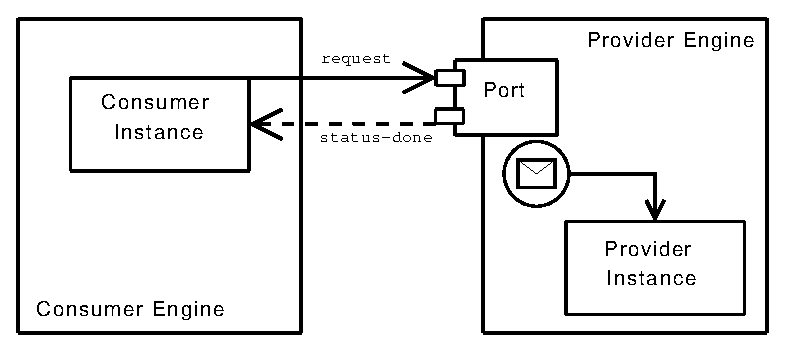
\includegraphics
{architettura_interna/dia/oneway}
\caption[Comunicazione One-Way] {
   	Il modello di comunicazione One-Way realizzato dai Blite
   	Engine.}
   	\rule{7cm}{0.01cm}
  \label{fig:oneway}
\end{center}
\end{figure}


Tele modello ci \`e sembrato il più adatto per poter realizzare i 
comportamenti seguenti:

\begin{itemize}
  \item Una istanza di processo può invocare operazioni di altri servizi in
  maniera asincrona potendo continuare a svolgere altre attività mentre
  l'elaborazione remota \`e in atto.
  
  \item Se un'istanza invoca un servizio che non esiste, o che \`e
  momentaneamente indisponibile o con modalità non conformi, l'istanza deve
  essere ricevere notifica di tale accadimento.
\end{itemize}

Di fatto questo c'\`e sembrato il giusto compromesso fra una comunicazione
sincrona (che del resto può sempre essere riprodotta) e una comunicazione puramente
``fire-and-forget'' come specificato nella semantica originale di Blite, in cui le
istanze procedono i maniera totalmente svincolata senza poter fare nessuna ipotesi sull'esito della comunicazione. Inoltre questo
modello di comunicazione \`e quello che meglio si adatta al binding su
protocolli di trasporto tipo HTTP, in cui ad una richiesta c'è sempre una
risposta del server che chiude la connessione. In HTTP una invocazione remota 
secondo lo scema One-Way può essere implementata come segue:

\begin{itemize}
  \item il client esegue una \emph{HTTP GET} o \emph{HTTP POST}
  \item il server risponde con \emph{202 Accepted}, nel caso il messaggio possa
  essere accettato, o con un error code della serie 400 o 500 (es. 400 Bad
  Request), nel caso in cui ci sia una qualche problema con la richiesta
  ricevuta.
\end{itemize}


Per concludere questa sezione facciamo vedere come lo schema di comunicazione
One-Way può essere facilmente realizzato con il modello ad eventi previsto
dalla nostra architettura. Per far questo riportiamo i passi logici eseguiti
dal componente \icode{InvokeActivity}:

\begin{enumerate}
  \item Si costruisce il messaggio e l'oggetto \icode{MessageConteniner}, 
  utilizzato per inviare il messaggio stesso nell'\icode{EngineChanel} (si
  veda la Sezione \ref{sec:progmot}). Si crea un identificativo del Service Provider
  tramite il seguente metodo messo a disposizione dell'interfaccia del ProcessManager:
  \begin{lstlisting}
  	/**
     * Resolve PartnerLink at rintime.
     * 
     * @param partnersmDef Static definition of the PartnerLink
     * @param variableScope Runtime variable scope
     * 
     * @return ServiceIdentifier the runtime partner link.
     */
    public ServiceIdentifier resovleParterLink(BLTDEFInvPartners partnersDef, 
											   VariableScope variableScope);
    
  \end{lstlisting}  
  
  \item Tramite il seguente metodo: 
  \begin{lstlisting}
  	InComingEventKey invoke(ServiceIdentifier serviceId, String operation, 
							MessageContainer messageContainer);
  \end{lstlisting}
  fornito dalla interfaccia del \icode{ProcessManager}, si avvia la
  comunicazione. Si osservi che il metodo restituisce un oggetto
  \texttt{eventKey} rappresentante come sempre una chiave di tipo \icode{InComingEventKey}. Nel caso particolare sarà un oggetto della classe
  \icode{StatusInComingEventKey} che individuerà l'arrivo dello status
  associato alla richiesta. Questo tipo di chiavi verranno generate a livello di
  Environment negli strati di più basso livello e le caratteristiche di unicità dipenderanno fortemente dalla tecnologia di comunicazione
 utilizzata. Per esempio nell'ambito della tecnologia JBI \cite{JBI} tali chiavi
 potranno coincidere con i \icode{MessgeaExchange}, mentre in ambito puramente
 TCP potranno essere ricavate dagli identificativi di connessione. In ogni modo a livello di Engine
 \`e possibile astrarre (e lo si deve fare) completamente dalla loro natura e
 utilizzarle semplicemente come identificatori univoci di eventi.
  
  \item In sezione critica sul monitor \icode{DefinitionProcessLevelLock}, si
  prova a consumare l'evento associato all'\texttt{eventKey}. Se questo \`e
  effettivamente già disponibile si valuta lo status di ritorno. Se si \`e
  avuto uno \texttt{status-done} si termina l'attività mettendo come
  attività corrente del FlowExecutor il parentComponet e si restituisce
  \texttt{true}, se invece si \`e avuto \texttt{status-error} si avvia la
  procedura di errore. Se l'evento associato all'\texttt{eventKey} non fosse
  ancora disponibile si registra il FlowExecutor come in attesa dello stesso e
  si termina il metodo \icode{doAtivity()} restituendo \texttt{false}.
  
  \item Quando l'evento atteso sarà disponibile il FlowExecutor verrà
  risvegliato e l'invokeActivity potrà essere di nuovo messa in esecuzione.
  Questa, disponendo già di \texttt{eventKey}, potrà rendersi conto di aver
  già eseguito l'invocazione e potrà semplicemente consumare l'evento
  atteso e procedere nell'analisi dello status come descritto sopra. Si
  osservi che in questo caso non sarà necessario operare in sezione critica.
\end{enumerate}

% %%%%%%%%%%%%%%%%%%%%%%%%%%%%%%%%%%%%%%%%%%%%%%%%%%%%%%%%%%%%%%%%%%%%%%%%%%%%%%%
% CONTESTI E COMPESAZIONE
% %%%%%%%%%%%%%%%%%%%%%%%%%%%%%%%%%%%%%%%%%%%%%%%%%%%%%%%%%%%%%%%%%%%%%%%%%%%%%%%
\section{Contesto, FaultHandler e Compensazione}

Il contesto è senz'altro quello uno dei costrutti più caratteristici di BPEL.
Tale costrutto \`e stato riprodotto con le opportune semplificazioni anche in
Blite e nella versione qui implementata.

Semplificando e rimanendo nell'ambito del linguaggio da noi implementato, un
contesto \`e un raggruppamento logico di attività (di fatto realizzato da
quella che indicheremo con \emph{ContextActivity}), a cui possono essere
associati un \emph{FaultHandler} e un \emph{CompensationHandler}\footnote{Nel
caso in cui il programmatore non codifichi direttamente gli Handler, sono
previste due versioni di default. Il DefaultFaultHandler prevede
semplicemente la ThrowActivity, in questo modo si lascia la gestione
dell'eccezione al contesto di livello superiore, mentre il
DefaultCompensationHandler prevede la semplice EmptyActivity.}. I due handler
non sono altro che due attività, la \emph{FaultHandlerActivity} e la \emph{CompensationHandlerActivity} che hanno funzionalità in un certo senso complementari.

\begin{itemize}
  \item La FaultHandlerActivity, \`e un'attività che deve essere eseguita nel
  caso in cui sia sollevato un Fault non gestito 
  durante l'esecuzione della ContestActivity. Di fatto si può pensare che la
  ContestActivity non sia stata completata a causa del verificarsi di una 
  situazione di errore e che a livello del contesto di definizione della 
  ContestActivity stessa si possa gestire l'errore tramite l'esecuzione della 
  FaultHandlerActivity. Quindi la FaultHandlerActivity entra in gioco nel
  momento in cui la ContestActivity non completa.
  
  \item Al contrario, CompensationHandlerActivity entra in gioco solo nel caso
  in cui ContestActivity completi la propria esecuzione con successo, cioè
  senza che si siano verificati errori non gestiti. Di fatto la
  CompensationHandlerActivity può essere vista come una serie di operazioni
  capaci di annullare ciò che \`e stato fatto dalla ContestActivity nel suo
  complesso. 
  Supponiamo di avere un contesto \texttt{c2}, a sua volta
  contenuto in un contesto \texttt{c1} (cioè \texttt{c2} \`e una sotto
  attività di \texttt{a1}, ContestActivity di \texttt{c1}), e che
  \texttt{c2} definisca la ContestActivity \texttt{a2} e la CompensationHandlerActivity
  \texttt{ch1}. Nel caso in cui \texttt{a2} completi con successo la sua
  esecuzione, \texttt{ch2} verrà resa nota a \texttt{c1} che la potrà
  utilizzare per annullare gli effetti di \texttt{a2} qualora si verifichi
  qualche successivo errore che impedisca a \texttt{a1} di completare con
  successo.
   
\end{itemize}

Da quanto detto si capisce che l'esecuzione degli handler di un contesto
\texttt{c} \`e strettamente legata al verificarsi di situazioni di errori:
la FaultHandlerActivity \`e lanciata qualora si verifichi un'eccezione
nell'esecuzione della ContestActivity di \texttt{c} stesso, la
CompensationHandlerActivity \`e lanciata qualora completato \texttt{c} si
verifichi un errore nell'esecuzione di una qualche attività ``sorella'' di
\texttt{c} \footnote{Nell'ambito della sintassi e semantica di Blite
l'espressione ``attività sorella'' ha il seguente significato: ``attività che \`e eseguita
nel medesimo contesto immediatamente contenente il contesto \texttt{c}''.}.

Il verificarsi di un'eccezione, oltre a mettere in esecuzione le eventuali
CompensationHandlerActivity e FaultHandlerActivity associate, ha un altro
effetto: la terminazione di tutti i flussi ``fratelli'' o discendenti dei
fratelli del flusso in cui si genera il fault. Per capire gli effetti prodotti dal
verificarsi di un'eccezione si faccia riferimento alla Figura \ref{fig:fault}
dove \`e rappresentato il seguente scenario a runtime:

\begin{itemize}
  \item Il contesto base \texttt{C0} definisce il FaultHandler \texttt{fh0}.
  \item L'esecuzione della ContestActivity di \texttt{C0} produce tre flussi di
  esecuzione parallela \texttt{f1}, \texttt{f2} e \texttt{f3}.
  \item Nel flusso \texttt{f1} viene eseguito in contesto \texttt{C1} che
  termina, installando in \texttt{C0} il CompensationHandler \texttt{ch1}.
  \item Nel flusso \texttt{f2} vine creato un nuovo contesto \texttt{C2}.
  All'interno del quale un FlowActivity avvia altri due flussi paralleli
  \texttt{f4} e \texttt{f5}.
  \item Nell'esecuzione del flusso \texttt{f3} viene generato un fault che
  dovrà essere gestito a livello del cotesto \texttt{C0}.
  \item Il fault produce la terminazione dei flussi \texttt{f1} e \texttt{f2} e
  a cascata dei flussi \texttt{f4} e \texttt{f5}.
  \item Il fault produce la creazione di un contesto protetto in cui saranno
  eseguite in sequenza la CompensationHandlerActivity \texttt{ch1} e la
  FaultHandlerActivity \texttt{fh0}.
\end{itemize}

\begin{figure}[t]
\begin{center}
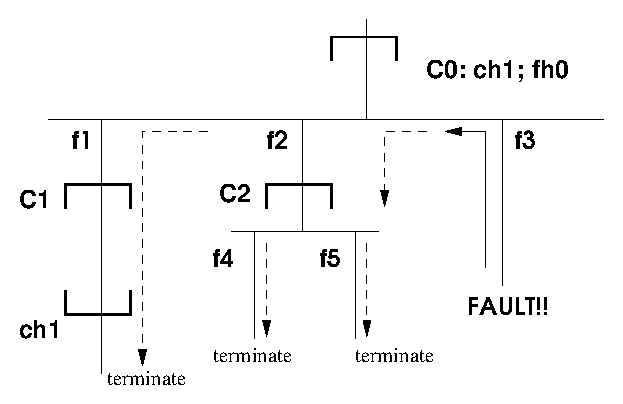
\includegraphics
{architettura_interna/dia/fault}
\caption[Propagazione di un'eccezione] {
   	Un'eccezione sollevata in un flusso di esecuzione produce la
   	terminazione di tutti i flussi paralleli e la conseguente messa in
   	esecuzione di Compensation Handler istallati e FaultHandler definiti nel
   	Contesto padre dei flussi.}
   	\rule{7cm}{0.01cm}
  \label{fig:fault}
\end{center}
\end{figure}

Come si può vedere dalla Figura \ref{fig:fault} la notifica e gli effetti di un
fault si propagano nelle due direzioni opposte nella gerarchia a runtime delle
attività. Dall'attività che ha scatenato il fault, risalendo i padri, raggiunge
il primo contesto e da questo riscende verso le attività figlie per
interrompere i vari flussi paralleli. Questo andamento di salita e discesa dell'informazione,
legata al verificarsi di una eccezione, \`e la caratteristica peculiare della
semantica di BPEL e quindi di Blite, e sulla base di questa caratteristica sono
stati disegnati le componenti e le interfacce software dell'Engine predisposte
alla gestione dei contesti e delle eccezioni.
\\

L'entità principale designata per la realizzazione dei meccanismi esposti \`e
stata individuata nel \icode{ExecutionContext}, la cui interfaccia, citata più
volte nelle sezioni precedenti, è presentata nel Listato
\ref{lst:ExecutionContext}. In particolare si \`e visto che un oggetto conforme a
tale interfaccia era presente nella segnatura del metodo
\icode{makeRuntimeActivity()} della classe \icode{ActivityComponentFactory}.
Difatti ogni oggetto ActivityComponent nascerà all'interno di un contesto di
esecuzione ExecutionContext. Le classi concrete che implementano l'interfaccia
ExecutionContext sono tre, come si vede dalla Figura \ref{fig:cntxclass}: la
\icode{ProcessInstanceImp}, la \icode{ScopeActivity} e la \icode{ProtectedScope}.
Ogni istanza di processo infatti costituirà il contesto base per una esecuzione e
all'interno di esso le varie attività ScopeActivity andranno a realizzare dei
sottocontesti. Un discorso a parte invece merita il tipo ProtectedScope, che
permette di realizzare speciali contesti, ``protetti'', in cui come si è visto
dovranno essere eseguiti i Fault e Compensation Handler. Ancora una volta per
fattorizzare i comportamenti comuni si \`e definita una classe astratta
\icode{ABaseContext} in cui è codificata gran parte della specifica
dell'interfaccia ExecutionContext.

\begin{figure}[t!]
\begin{center}
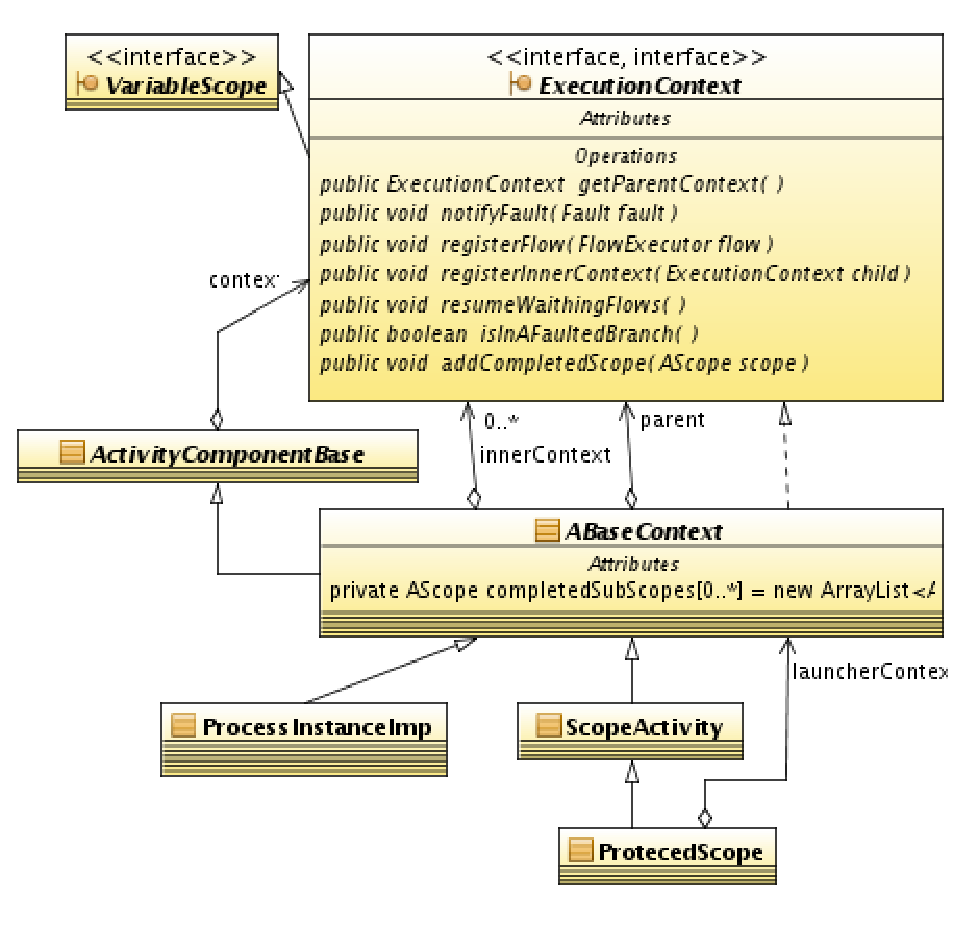
\includegraphics[scale=0.85]
{architettura_interna/dia/cntxclass}
\caption[ExecutionContext Class Diagram]{
   	\icode{ABaseContext} e le sue sottoclassi forniscono 
   	diverse implementazioni dell'interfaccia	\icode{ExecutionContext} }
   	\rule{7cm}{0.01cm}
  \label{fig:cntxclass}
\end{center}
\end{figure}

In pratica le varie attività che implementano l'Interfaccia ExecutionContext
realizzano una sotto gerarchia all'interno della gerarchia principale delle
ActivityComponent. Infatti, a parte la ProcessInstance che costituisce la
radice dell'albero, ogni ExecutionContext avrà un \icode{parentContext} ed
eventualmente un insieme di contesti figli.

\lstinputlisting[caption={Interfaccia \icode{ExecutionContext}.},
label=lst:ExecutionContext]{architettura_interna/java/ExecutionContext.java}

In Tabella \ref{it:ExecutionContext} analizziamo l'interfaccia
\icode{ExecutionContext} nei suoi metodi principali, mentre di seguito vediamo
come questi possono essere utilizzati per realizzare la semantica specificata.

\begin{table}[h!]
\begin{tabular}{| p{0.42\textwidth } | p{0.52\textwidth}|}
\hline
\icode{ExecutionContext} &  \\

\hline
\small{\icode{ExecutionContext getParentContext()}} & \small{Restituisce il contesto padre
del contesto corrente}\\

\hline
\small{\icode{void registerInnerContext( \hspace*{\stretch{2}} \linebreak  
\hspace*{\stretch{3}} ExecutionContext child)}} & \small{Aggiunge un
contesto figlio al contesto corrente}\\

\hline
\small{\icode{void 
notifyFault(Fault fault)}} & \small{Con questo metodo \`e
possibile sollevare eccezioni (faults). Le attività che necessiteranno di
lanciare eccezioni (per esempio la \icode{ThrowActivty}) potranno invocare
tale metodo su il loro ExecutionContext e terminare il loro metodo
\icode{doActivity} rimettendo in esecuzione il loro parentComponent.
L'ExecutionContext potrà aggiornare il proprio stato per riflettere la situazione di errore.
Con questo metodo ha inizio la propagazione del fault.}\\

% \end{tabular}
% \begin{tabular}{| p{0.45\textwidth } | p{0.55\textwidth}|}


\hline \small{\icode{boolean isInAFaultedBranch()}} & \small{Questo
metodo sarà utilizzato da ogni attività per vedere se nella loro gerarchia di
contesti ne sia presente uno su cui sia stata notificata un'eccezione. La
gerarchia in questo caso sarà ispezionata dal contesto padre verso i
predecessori. In tal caso, le attività dovranno collaborare per attuare la
terminazione del proprio flusso, cioè dovranno terminare mettendo in
esecuzione  il proprio \icode{parentComponent}.}\\


\hline \small{\icode{void registerFlow(FlowExecutor flow)}} & \small{
Poiché il processo di terminazione deve coinvolgere tutti i flussi, anche quelli che eventualmente
sono in attesa di eventi, il contesto, una volta notificato del fault, dovrà
risvegliare tutti i flussi creati sotto lui per far si che questi possano
terminare. Ovviamente, per poter far questo, il contesto dovrà conoscere i
flussi che sono stati creati sotto di lui. Con questo metodo di fatto si realizza
proprio questo, si metterà a conoscenza il contesto sotto cui si sta operando
di ogni nuovo flusso creato. }\\

% \hline
% \small{void \textbf{resumeWaithingFlows}()} & \small{\textsf{}}\\

\hline
\small{\icode{void addCompletedScope(  \hspace*{\stretch{3}} \linebreak
\hspace*{\stretch{3}} AScope scope)}} & \small{Con questo metodo i
contesti completati con successo potranno registrare nel proprio contesto
padre il loro CompensationHandler per un eventuale esecuzione futura.}\\

\hline
\end{tabular}
\caption{Interfaccia \icode{ExecutionContext}}
\label{it:ExecutionContext}
\end{table}

Come abbiamo già osservato si \`e scelto un modello di esecuzione Activity
Centric, nel senso che le varie attività saranno totalmente responsabili nel
realizzare la loro esecuzione, ma anche nel collaborare per far sì che i flussi
globali dei processi evolvano secondo quanto specificato dalla semantica.
Nell'ambito della terminazione questo concetto si esemplifica nel fatto che ogni
attività (con la sola esclusione delle attività \emph{short-lived}) ogni
qualvolta venga eseguita, dovrà per prima cosa verificare se si stia trovando
nella discendenza di un contesto fallito (questo potrà essere verificato
invocando il metodo \icode{isInAFaultedBranch()} del proprio ExecutionContext).
In caso di risposta positiva l'attività dovrà collaborare alla terminazione del
proprio flusso di esecuzione, cioè dovrà impostare il proprio
\icode{parentComponent} come attività corrente del FlowExecutor e concludere
immediatamente il metodo \icode{doActivity()} restituendo il valore true. In
questo modo, con un processo a catena, il flusso corrente raggiungerà il
FlowOwner e potrà così terminare.
\\

Di fatto la ricerca di un fault a ritroso nella gerarchia dei contesti può
essere semplicemente fatta implementando il metodo \icode{isInAFaultedBranch()}
secondo il seguente algoritmo ricorsivo\footnote{Quella qui presenta \`e
l'implementazione fornita dalla classe ABaseContext ereditata anche per i
contesti ProcessInstanceImp e ScopeActivity. Come si vedrà, il contesto
ProtectedScope invece, fornisce una riscrittura di questa implementazione per
garantire la protezione dell'esecuzione.}:

\begin{enumerate}
  \item Se lo stato corrente del contesto \`e uguale a \texttt{FAULTED} (cioè
  al contesto \`e stato notificato direttamente un fault) si restituisce
  \texttt{true}. Altrimenti si procede al passo successivo.
  \item Se il contesto non ha un contesto padre si restituisce \texttt{false}.
  Altrimenti si procede al passo successivo.
  \item Ricorsivamente si restituisce il valore restituito dal metodo 
  \icode{isInAFaultedBranch()} invocato sul contesto padre.
\end{enumerate}

\`E anche interessante osservare quale è la procedura alla
base dell'implementazione del metodo \icode{notifyFault(Fault
fault)}\footnote{Anche questa implementazione \`e fornita dalla classe ABaseContext ed \`e conforme
alla semantica dei contesti ProcessInstanceImp e ScopeActivity. Per il contesto
ProtectedScope come si vedrà è necessario una piccola modifica.}:

\begin{enumerate}
  \item Si imposta lo stato interno al valore \texttt{FAULTED}.
  \item Si invoca sul contesto corrente il metodo \icode{resumeWaitingFlows()}.
  Tale metodo ha un comportamento ricorsivo:
  \begin{itemize}
  	\item  Su ogni contesto figlio del contesto corrente si invoca ricorsivamente
  	il metodo \icode{resumeWaitingFlows()} stesso.
  	\item Si risveglia il ogni flusso di esecuzione registrato nel contesto
  	corrente. Tale operazione viene fatta in sezione critica sul consueto
  	semaforo disponibile a livello di definizione di processo:
	%\lstset{frame=NONE}  	
	\begin{lstlisting}
	synchronized (manager.getDefinitionProcessLevelLock()) {
                engine.resumeWaitingFlow(flow);
    }
  	\end{lstlisting}	  	 
  \end{itemize}
\end{enumerate}

Le due implementazioni saranno valide sia per i contesti di tipo
ProcessInsatnceImp che per i contesti definiti dalle ScopeActivity. In più, il
metodo \icode{doActivity()} di quest'ultima classe realizzerà un algoritmo del
tipo seguente:

\begin{itemize}
  \item Se \icode{isInAFaultedBranch()} \`e \texttt{true}:
  	\begin{itemize}
    	\item Se lo stato corrente \`e \texttt{FAULTED}, cioè il contesto ha
    	ricevuto direttamente notifica di un'eccezione, si devono avviare gli
    	Handler:
    		 \begin{itemize}
             	\item Si crea una SequenceActivity con la sequenza dei
             	CompensationHandler istallati e con il FaultHandler definito.
             	\item Si crea un ProtectedScope in cui si imposta come
             	ContestActivity la SequenceActivity appena creata.
             	\item Si imposta come attività corrente del FlowExecutor il
             	ProtectedScope e si restituisce il valore \texttt{true}.
             \end{itemize}    
    	\item Se lo stato corrente non \`e \texttt{FAULTED}, cioè un'eccezione
    	\`e stata notificata in un qualche contesto padre:
    		 \begin{itemize}
             	\item Si imposta lo stato a \texttt{TERMINATED}.
             	\item Si crea un ProtectedScope in cui si imposta come
             	ContestActivity la sequenceActivity dei CompesationHandler
             	installati. 
             	\item Si imposta come attività corrente sul FlowExecutor la
                parentComponent e si restituisce dal metodo con
                \texttt{true}
%                 \footnote{Bisogna osservare che questo
%                 comportamento \`e conforme alla semantica attuale di Blite in
%                 cui la terminazione di un contesto coincide con la terminazione
%                 della sua ContestActivity. In realtà se si volesse essere più
%                 fedeli alla filosofia BPEL e forse più in linea con le
%                 aspettative di un ipotetico utente del linguaggio, la
%                 terminazione di un contesto dovrebbe prevedere la messa in
%                 esecuzione dei CompensationHandler attualmente istallati nel
%                 contesto stesso. Questo del resto \`e anche il comportamento
%                 dei default TerminationHandlers di BPEL.}
				.
             \end{itemize}
    \end{itemize}    
  
  \item Altrimenti, cioè se \icode{isInAFaultedBranch()} è \texttt{false}:
  	\begin{itemize}
  		\item Se lo stato corrente \`e \texttt{STARTED}, cioè uguale allo stato
  		iniziale all'attività, il contesto deve iniziare l'esecuzione, per cui:
  			\begin{itemize} 
                \item Si imposta lo stato a \texttt{RUNNING}.
                \item Si mette come attività corrente del FlowExecutor la
                ContestActivity e si ritorna con \texttt{true}.
        	\end{itemize}   
  		\item Se lo stato corrente \`e \texttt{RUNNING} allora la ContestActivity
  		ha completato correttamente la sua esecuzione:
  			\begin{itemize} 
                \item Si imposta lo stato a \texttt{COMPLETED}. 
                \item Si registra il CompensationHandler nel contesto padre.
                \item Si imposta come attività corrente sul FlowExecutor la
                \icode{parentComponent} e si restituisce dal metodo con
                \texttt{true}.
        	\end{itemize}  		 
	\end{itemize}
\end{itemize} 


Concludiamo questa sezione analizzando il contesto \icode{ProtectedScope}. Come
già detto tale contesto è utilizzato per la messa in esecuzione dei
CompesationHandler e dei FaultHandler di un contesto oggetto di un fault.
La semantica di Blite caratterizza tali contesti, differenziandoli da quelli
definiti dalle ScopeActivity, solo per il fatto che questi sono immuni alla
terminazione o se si vuole parlare in termini della semantica Blite, la
funzione {\sf{end($\cdot$)}} agisce come la funzione identità per questi
contesti:

$$
\sf{ end( \, \llparenthesis a \rrparenthesis \, ) = \llparenthesis a
\rrparenthesis }
$$
 
Questa caratterizzazione è implementata nel nostro modello andando a
riscrivere il metodo \icode{isInAFaultedBranch()} nella classe ProtectedScope in
modo tale da evitare la chiamata ricorsiva sui contesti padre. Di fatto
l'implementazione in questo caso seguirà il seguente semplice schema:

\begin{itemize}
  \item Se lo stato corrente del contesto \`e uguale a \texttt{FAULTED} (cioè
  sul contesto \`e stato notificato direttamente un fault) si restituisce
  \texttt{true}. Altrimenti 
  \item Si restituisce \texttt{false}.
\end{itemize}

In questo modo l'esecuzione che avviene in un ExecutionContext di tipo
ProtectedScope \`e protetta dai fallimenti che possono avvenire in altri flussi
paralleli. 
\\

Un'altra caratteristica della semantica di Blite \`e che il ProtectedScope
protegge l'attività interna dai fallimenti esterni, ma non fa il viceversa, cioè i
fallimenti che avvengano all'interno del ProtectedScope si propagano verso il
contesto in cui il ProtectedScope \`e eseguito. Nel momento in cui il
ProtectedScope viene creato, in fase di gestione dell'eccezione, il contesto
fallito imposta il proprio contesto padre come contesto padre del ProtectedScope
stesso; a questo punto la ``semi trasparenza'' definita dalla semantica di Blite
per il ProtectedScope, si realizza nel momento in cui il metodo
\icode{notifyFault(Fault fault)} viene riscritto secondo la seguente logica:

\begin{itemize}
  \item Si imposta lo stato a al valore \texttt{FAULTED},
  \item Si invoca lo stesso metodo notifyFault(fault) su parentContext
	%\lstset{frame=NONE}
	\begin{lstlisting}
		@Override
   		public void notifyFault(Fault fault) {
        	setSate(ContextState.FAULTED);
        	getParentContext().notifyFault(fault);
    	}
  	\end{lstlisting}   
\end{itemize}

Si può facilmente capire che con questa implementazione il ProtectedScope è del
tutto trasparente per le eccezioni che avvengono al suo interno le quali si
propagano direttamente sul contesto padre dove eventualmente possono essere
anche gestite.
